\documentclass{article}
\usepackage{cmap}
\usepackage[T1,T2A]{fontenc}
\usepackage[utf8]{inputenc}
\usepackage[russian]{babel}
\usepackage[left=2cm,right=2cm,top=2cm,bottom=2cm,bindingoffset=0cm]{geometry}
\usepackage{tikz}
\usepackage{setspace,amsmath}
\usepackage{tabularx}
\usepackage{multirow}
\usepackage{makecell}
\usepackage{listings}
\usepackage{titlesec}
\usepackage{lipsum}
\usepackage[usestackEOL]{stackengine}
\usepackage{kantlipsum}
\usepackage{caption}
\usepackage{float}
\usepackage{fancyhdr}
\usepackage{graphicx}
\usepackage{hyperref}
\usepackage{eso-pic}
\hypersetup{hidelinks} % This hides the hyperlinks
\pagestyle{fancy}
\fancyhf{}
\fancyhead[C]{\thepage\\ RU.17701729.10.03-01 ВКР 01-1}
\renewcommand{\headrulewidth}{0pt}
\captionsetup[table]{justification=centering}
\usetikzlibrary{positioning}
\graphicspath{{pictures/}}
\DeclareGraphicsExtensions{.pdf,.png,.jpg}
\newcommand\zz[1]{\par{\normalsize\strut #1} \hfill\ignorespaces}
\addto\captionsrussian{\def\refname{}}
\newcommand{\subtitle}[1]{%
    \posttitle{%
        \par\end{center}
        \begin{center}\Large#1\end{center}
    }%
}
\newcommand{\subsubtitle}[1]{%
    \preauthor{%
        \begin{center}
        \large #1 \vskip0.5em
        \begin{tabular}[t]{c}
    }%
}
\newcommand{\mytable}{
    \AddToShipoutPictureBG*{%
        \begin{tikzpicture}[remember picture, overlay]
        \node[anchor=south west, xshift=1cm, yshift=1cm] at (current page.south west) {
            \begin{tabular}{|>{\raggedright\arraybackslash}m{0.3cm}|>{\centering\arraybackslash}m{0.3cm}|}
            \hline
            \rotatebox{90}{\textit{\textbf{Инв. № подл. }}} & \rotatebox{90}{} \\
            \hline
            \rotatebox{90}{\textit{\textbf{Подп. и дата }}} & \rotatebox{90}{} \\
            \hline
            \rotatebox{90}{\textit{\textbf{Взам. инв. № }}} & \rotatebox{90}{} \\
            \hline
            \rotatebox{90}{\textit{\textbf{Инв. № дубл. }}} & \rotatebox{90}{} \\
            \hline
            \rotatebox{90}{\textit{\textbf{Подп. и дата }}} & \rotatebox{90}{} \\
            \hline
            \end{tabular}
        };
        \end{tikzpicture}
    }
}
\begin{document}
    \thispagestyle{empty}
    \begin{center}
        \textbf{
            ПРАВИТЕЛЬСТВО РОССИЙСКОЙ ФЕДЕРАЦИИ\\
            НАЦИОНАЛЬНЫЙ ИССЛЕДОВАТЕЛЬСКИЙ УНИВЕРСИТЕТ\\
            «ВЫСШАЯ ШКОЛА ЭКОНОМИКИ»\\
            Факультет компьютерных наук\\
            Образовательная программа «Программная инженерия»\\
            (ВШЭ ФКН ПИ)}\\
    \end{center}
    \bigskip
    \zz{УДК 004.94:005.8}
    \zz{СОГЛАСОВАНО}УТВЕРЖДАЮ
    \zz{Доцент департамента}Академический руководитель
    \zz{Программной инженерии,}образовательной программы
    \zz{ФКН, к.т.н.}«Программная инженерия»
    \zz{\noindent\rule{3cm}{0.4pt} К. Ю. Дегтярёв}старший преподаватель
    \zz{«\noindent\rule{1cm}{0.4pt}»\noindent\rule{2cm}{0.4pt}20\noindent\rule{0.5cm}{0.4pt}г.}\noindent\rule{3cm}{0.4pt} Н. А. Павлочев
    \zz{}«\noindent\rule{1cm}{0.4pt}»\noindent\rule{2cm}{0.4pt}20\noindent\rule{0.5cm}{0.4pt}г.
    \begin{center}
        \topskip=0pt
        \vspace*{\fill}
        \textbf{Выпускная квалификационная работа}\\
        (академическая)\\
        на тему: \textbf{ПРОГРАММА ДЛЯ МОДЕЛИРОВАНИЯ ВОСПРИЯТИЯ\\
        ФАКТОРОВ УСПЕХА IТ-ПРОЕКТА С ИСПОЛЬЗОВАНИЕМ\\
        НЕЧЕТКИХ КОГНИТИВНЫХ КАРТ}\\
        ~\\
        по направлению подготовки 09.03.04 «Программная инженерия»\\
        \vspace*{\fill}
    \end{center}
    \zz{~}Исполнитель
    \zz{~}Студент группы БПИ204
    \zz{~}образовательной программы
    \zz{~}«Программная инженерия»
    \zz{~}Пеганов Никита Сергеевич
    \zz{~}\noindent\rule{3cm}{0.4pt} Н. С. Пеганов
    \zz{~}«\noindent\rule{1cm}{0.4pt}»\noindent\rule{2cm}{0.4pt}20\noindent\rule{0.5cm}{0.4pt}г.
    \begin{center}
        \vspace*{\fill}{
            Москва \the\year{}}
    \end{center}
    \mytable
    \newpage
    \clearpage
    \pagenumbering{arabic}
    \bigskip
    \bigskip
    \begin{center}
        \topskip=0pt
        \vspace*{\fill}
        \textbf{Выпускная квалификационная работа}\\
        (академическая)\\
        на тему: \textbf{ПРОГРАММА ДЛЯ МОДЕЛИРОВАНИЯ ВОСПРИЯТИЯ\\
        ФАКТОРОВ УСПЕХА IТ-ПРОЕКТА С ИСПОЛЬЗОВАНИЕМ\\
        НЕЧЕТКИХ КОГНИТИВНЫХ КАРТ}\\
        ~\\
        по направлению подготовки 09.03.04 «Программная инженерия»\\
        ~\\
        Листов \ztotpages\\
        \vspace*{\fill}
    \end{center}
    \begin{center}
        \vspace*{\fill}{
            Москва \the\year{}}
    \end{center}
    \mytable
    \newpage
    \tableofcontents
    \lefttable
    \newpage
    \section {Аннотация}
    В представленной пояснительной записке описывается работа программы "{}IT-success-factors-model.exe"{}, которая используется для моделирования восприятия факторов успеха IT-проекта с использованием метода нечетких когнитивных карт. Задачей данной программы является обеспечение возможности визуализации, анализа и понимания динамики развития IT-проектов посредством моделирования взаимного влияния ключевых факторов их успешности.\\
    ~\\
    Основные требования к содержанию и оформлению данной пояснительной записки разработаны в соответствии с:
    \begin{itemize}
        \item ГОСТ 19.101-77 Виды программ и программных документов \cite{litlink1};
        \item ГОСТ 19.102-77 Стадии разработки \cite{litlink2};
        \item ГОСТ 19.103-77 Обозначения программ и программных документов \cite{litlink3};
        \item ГОСТ 19.104-78 Основные надписи \cite{litlink4};
        \item ГОСТ 19.105-78 Общие требования к программным документам \cite{litlink5};
        \item ГОСТ 19.106-78 Требования к программным документам, выполненным печатным
        способом \cite{litlink6};
        \item ГОСТ 19.404-79 Пояснительная записка. Требования к содержанию и оформлению \cite{litlink7}.
    \end{itemize}
    Изменения к данной пояснительной записке оформляются согласно ГОСТ 19.603-78 \cite{litlink8}, ГОСТ 19.604-78 \cite{litlink9}.
    \lefttable
    \newpage
    \section {Введение}
    \subsection {Наименование программы на русском языке}
    Программа для моделирования восприятия факторов успеха IТ-проекта с использованием нечетких когнитивных карт.
    \subsection {Наименование программы на английском языке}
    A Program for Modeling the Perception of Success Factors of an IT-Project Using Fuzzy Cognitive Maps.
    \subsection {Документы, на основании которых ведется разработка}
    Программа разработана в рамках выполнения выпускной квалификационной работы — "{}Программа для моделирования восприятия факторов успеха IТ-проекта с использованием нечетких когнитивных карт"{}, в соответствии с учебным планом 4 курса бакалавриата направления 09.03.04 «Программная инженерия» \cite{litlink10}.\\
    ~\\
    Основание для разработки — учебный план подготовки бакалавров по направлению 09.03.04 «Программная инженерия» \cite{litlink11} и утвержденная академическим руководителем программы тема дипломной работы.
    \lefttable
    \newpage
    \section {Назначение и область применения}
    \subsection {Назначение программы}
    Общим назначением разрабатываемой программы является визуализация, анализ и понимание факторов успеха IT-проектов. Это достигается путем использования нечетких когнитивных карт, что позволяет включить в модель любые переменные (факторы), даже те, которые сложно или невозможно измерить в количественных терминах. Основное назначение этого ПО — определение и визуализация взаимосвязей между различными факторами с точки зрения стейкхолдеров.\\
    ~\\
    Программа реализует нечеткие модели вычислений, с помощью которых аналитики могут оценивать и анализировать полученные данные, опираясь на предложенные нечеткие модели вычислений. Нечеткие когнитивные карты (Fuzzy Cognitive Maps, FCM) дают возможность моделировать одну и ту же систему по-разному, в зависимости от целей и профессиональных навыков людей или групп людей, фиксируя изменяемые во времени величины моделируемой ситуации.\\
    ~\\
    Программа генерирует FCM, которые можно использовать для визуализации сложных систем и отображения их развития во времени. При этом, в ряде случаев, применяется SWOT-анализ — это позволяет более полно охарактеризовать исследуемые факторы.\\
    ~\\
    С течением времени, могут меняться не только сами факторы, но и связи между ними. Программа позволяет учесть это, перестраивая и модифицируя карты. Это обеспечивает возможность итеративной корректировки модели и поиск новых зависимостей и уязвимостей.\\
    \subsection {Целевая аудитория продукта}
    Целевой аудиторией данной программы являются, преимущественно, специалисты, работающие в IT-секторе, а именно аналитики, менеджеры проектов и IT-директора. Это связано с тем, что программа позволяет моделировать восприятие факторов успеха IT-проектов и может быть полезной для исследования и управления различными аспектами таких проектов.\\
    ~\\
    Вместе с тем, данная программа может быть использована в обучающих целях и обладает потенциалом быть полезной для студентов и преподавателей IT-специальностей, особенно для тех, кто изучает или преподает курсы, связанные с управлением IT-проектами, анализом данных, искусственным интеллектом или когнитивной наукой.\\
    ~\\
    Наконец, потенциальными пользователями данной программы могут быть и авторы научных исследований из области IT и когнитивистики. Она может оказаться полезной при изучении восприятия факторов, влияющих на успех IT-проектов, и при исследовании механизмов принятия решений в рамках таких проектов.\\
    ~\\
    В то же время, следует отметить, что оперировать данной программой могут преимущественно люди, обладающие нужным навыком и знаниями для работы с нечеткими когнитивными картами. Подразумевается использование программы одним аналитиком и множеством стейкхолдеров для создания результата коллективного обсуждения.\\
    \subsection {Актуальность проблемы}
    В последнее время, в свете растущей зависимости бизнеса от технологий, успешное выполнение IT-проектов становится особенно важным для организаций различных сфер деятельности и масштаба. Однако, измерение и предсказание успеха в случае IT-проектов всё ещё являются сложной задачей, так как они зависят от множества факторов, характеризуемых неоднозначностью и взаимной связью с другими аспектами рассмотрения.\\
    ~\\
    \lefttable
    В связи с этим, программа для моделирования восприятия факторов успеха IT-проектов с использованием нечетких когнитивных карт обретает значительную актуальность. Факторы успеха проекта часто являются нечетко определенными и интерпретируемыми, что делает использование нечетких когнитивных карт подходящим выбором для их анализа и моделирования.\\
    ~\\
    Методология когнитивного моделирования была предложена американским политологом и экономистом Робертом Аксельродом \cite{litlink12}. Когнитивное моделирование предназначалось для принятия решений в плохо определенных ситуациях. Нечеткие когнитивные карты, впервые предложенные Бартом Коско \cite{litlink13}, являются смешанным типом графического представления знаний, включающего в себя элементы когнитивных карт и нечеткой логики.\\
    ~\\
    В последние годы они вновь привлекают внимание исследователей, подобно тому как нейронные сети после своего «забвения» в 90-х годах 20-го века, сейчас снова переживают свой пик популярности. Например, нечеткие когнитивные карты используются в исследовательских работах, написанных в 2018, 2019 и 2022 годах \cite{litlink14, litlink15, litlink16}. Как и нейронные сети, нечеткие когнитивные карты могут быть применены для моделирования сложных взаимосвязей и получения результатов на основе неопределенной и нечеткой информации.\\
    ~\\
    В многочисленных исследовательских работах авторы рассматривают нечеткие когнитивные карты как удобный и наглядный аппарат моделирования. Факторы и связи между факторами располагаются в FCM в стуктуре, подобной структуре головного мозга человека (в очень упрощенном виде), поэтому получаемая модель легко воспринимается и удобна для обсуждения. Также нечеткие когнитивные карты отличаются универсальностью, что позволяет использовать их в множестве различных областей \cite{litlink17}.\\
    ~\\
    Несмотря на нейросетеподобную структуру нечетких когнитивных карт, в рамках данной выпускной квалификационной работы не предполагается использование сложных алгоритмов нейронных сетей. Главным образом, это обусловлено спецификой выбранной методологии — нечетких когнитивных карт. Данный подход предполагает создание модели с использованием сетевой структуры, раскрывающей прямые и обратные связи между различными факторами успеха IT-проекта.\\
    ~\\
    Моделирование факторов успеха IT-проекта — одна из областей, в которых успешно применяются нечеткие когнитивные карты. Например, в работе "{}Modelling IT projects success with Fuzzy Cognitive Maps"{} \cite{litlink18} авторы применяют FCM для моделирования факторов успеха мобильной платежной системы, проекта, связанного с быстро развивающимся миром мобильных телекоммуникаций. Описанная в работе методология использует четыре матрицы для представления результатов, которые методология обеспечивает на каждом из своих этапов. Это начальная матрица успеха (IMS), Фаззифицированная матрица успеха (FZMS), Матрица успеха силы отношений (SRMS) и Итоговая матрица успеха (FMS). Авторы статьи делают вывод, что Критические факторы успеха (CSF) — это те необходимые условия, которым должен удовлетворять проект, чтобы его воспринимали как успешный. Требуется улучшение процессов определения и оценки подходящих CSF для ИТ-проектов из-за возросшей сложности и неопределенности.\\
    ~\\
    В работе "{}Using cognitive maps for modeling project success"{} \cite{litlink19}, вышедшей в том же году, применяются когнитивные карты. Для наглядности в ней рассматривается реальный строительный проект, реализованный в Турции. В работе также описаны приемущества и недостатки когнитивных карт. Среди преимуществ когнитивных карт авторы отмечают их способность представлять сложные идеи и информацию в простой и понятной форме. Когнитивные карты также помогают улучшить понимание и организацию знаний, а также способствуют более эффективному принятию решений. Однако у когнитивных карт также есть недостатки. Они могут быть сложными для создания и интерпретации, особенно если они включают большое количество информации или сложные взаимосвязи. Кроме того, они могут быть субъективными, поскольку они основаны на знаниях и восприятии отдельного человека или группы людей.\\
    ~\\
    В статье "{}Assessing it projects success with extended fuzzy cognitive maps \& neutrosophic cognitive maps in comparison to fuzzy cognitive maps"{} \cite{litlink20} представлено исследование, в котором авторы сравнивают применение расширенных нечетких когнитивных карт и нейтрософских когнитивных карт в оценке успеха проекта мобильной платежной системы. Для этого они создали различные когнитивные карты с несколькими группами стейкхолдеров. В результате, авторы сделали вывод, что нейтрософские когнитивные карты показали лучшие результаты, чем нечеткие когнитивные карты и улучшенные когнитивные карты.\\
    ~\\
    Анализ литературы показывает, что использование когнитивных карт является эффективным инструментом для моделирования и оценки факторов успеха IT-проектов. Эти методы позволяют представить сложные идеи и информацию в простой и понятной форме, улучшить понимание и организацию знаний, а также способствуют более эффективному принятию решений.\\
    ~\\
    Однако, как отмечено в анализируемых работах, эти методы имеют свои недостатки, включая сложность создания и интерпретации карт, особенно при большом объеме информации и сложных взаимосвязях, а также субъективность, поскольку они основаны на знаниях и восприятии отдельного человека или группы людей.\\
    ~\\
    Также стоит отметить, что важность определения и оценки критических факторов успеха (CSF) для IT-проектов подчеркивается во всех рассмотренных работах. Это подтверждает актуальность нашего исследования и выбранной темы выпускной квалификационной работы.\\
    ~\\
    Таким образом, разработка и использование программы для моделирования восприятия факторов успеха IT-проектов с использованием нечетких когнитивных карт является полезным и актуальным подходом к решению сложной проблемы IT-управления и планирования.\\
    \subsubsection {Функциональное назначение}
    Программа предназначена для моделирования восприятия различных факторов, которые способствуют или препятствуют успеху IT-проектов. Она использует принципы нечетких когнитивных карт для преобразования качественных оценок в количественные данные, что позволяет более точно анализировать и визуализировать динамику проекта.\\
    ~\\
    Основные функции программы включают:
    \begin{itemize}
        \item Создание списка факторов, влияющих на итоговый успех проекта. Эти факторы могут быть определены пользователем или группой пользователей, что обеспечивает гибкость системы и возможность учета уникальных особенностей каждой отдельной ситуации.
        \item Ввод данных о том, как каждый фактор влияет на другие, и преобразование этих данных в формальный вид с использованием нечетких множеств.
        \item Визуализация связей между факторами и расчет относительных значений в узлах, что позволяет увидеть, какой фактор является решающим и как он влияет на общую картину.
        \item Генерация выводов на основе анализа ситуации и формирование выводов о будущем ходе проекта.
        \item Запись и чтение созданных нечетких когнитивных карт в файл.
    \end{itemize}
    Таким образом, данная программа служит инструментом для анализа и улучшения процесса управления IT-проектами, позволяя более эффективно определять стратегии развития и принимать управленческие решения.
    \subsubsection {Эксплуатационное назначение}
    Эксплуатационное назначение разработанной программы заключается в моделировании восприятия влияния различных факторов на успех IT-проекта с использованием нечетких когнитивных карт.\\
    ~\\
    Программа предназначена для:
    \begin{itemize}
        \item Представления с каждым фактором определенной характеристики, которая помогает оператору понимать важность и актуальность данного фактора для проекта в целом;
        \item Возможности наблюдения и анализа весов связей между различными факторами, что позволяет оператору определить ключевые связи и элементы в структуре проекта;
        \item Предоставления информации о динамике изменения значений различных факторов во времени, что позволяет оператору реагировать на изменения во внешнем и внутреннем окружении проекта вовремя и принимать корректировки в стратегию проекта при необходимости;
        \item Выделения наиболее значимых факторов для успеха проекта, что позволяет сфокусироваться на ключевых элементах и не тратить ресурсы на менее важные аспекты;
        \item Получения дополнительной информации для лучшего понимания тех аспектов, которые в значительной или несущественной степени влияют на успех проекта.
    \end{itemize}
    Для каждого фактора учитывается гибкость настроек его влияния, относительные значения в узлах и влияние на другие факторы. Программа позволяет преобразовать оценки влияния с использованием нечеткой логики и формальных представлений нечетких множеств.\\
    ~\\
    Результатами работы программы становятся визуализированные когнитивные карты, на основе которых можно сделать выводы о наиболее важных моментах и факторах успеха IT-проекта.\\
    ~\\
    Одним из важных преимуществ программы является возможность имитации изменения взаимодействия факторов во времени, что позволяет проследить эволюцию проекта в долгосрочной перспективе.
    \subsection {Область применения программы}
    Программа для моделирования восприятия факторов успеха IT-проекта с использованием нечетких когнитивных карт предназначена для использования IT-специалистами, управляющими и исследователями в области управления информационными технологиями.\\
    ~\\
    Основные области применения программы включают:
    \begin{itemize}
        \item Разработку и управление IT-проектами. Моделирование факторов успеха проекта помогает управляющим эффективно управлять ресурсами и контролировать процесс реализации проекта;
        \item Исследование в области IT. Использование нечетких когнитивных карт позволяет формировать более точное и объективное представление об исследуемых объектах и процессах;
        \item Образование. Программа может быть использована для обучения студентов и участников профессиональных курсов основам управления IT-проектами и технологиям моделирования;
        \item Использование в комплексе с другими методами управления и предсказания для увеличения точности анализа и принятия решений.
    \end{itemize}
    Таким образом, данная программа может быть применена в различных областях связанных с IT-технологиями, включая научные исследования, обучение, планирование и управление IT-проектами.

    \newpage
    \section {Технические характеристики}
    \subsection {Постановка задачи на разработку программы}
    Разрабатываемая программа должна быть наделена следующими функциями:
    \begin{enumerate}
        \item  Обеспечивать оператору механизмы для создания моделей влияния факторов успеха IT-проекта, основываясь на предоставленных им данных и применяя метод нечетких когнитивных карт;
        \item  Давать возможность оператору создавать свои индивидуальные модели влияния действующих факторов на успех IT-проекта;
        \item  Позволять оператору выбирать факторы IT-проекта из списка существующих, наиболее часто встречающихся факторов;
        \item  Реализовывать функционал, позволяющий вносить изменения в построенные модели, в том числе добавлять или удалять факторы, изменять взаимосвязи между факторами и так далее;
        \item  Давать возможность оператору сохранять построенные или измененные модели во внешний файл;
        \item  Предоставлять возможность оператору сохранять разные версии когнитивной карты в процессе изменения;
        \item  Обеспечивать оператору возможность анализа информации о взаимосвязях факторов в различных вариантах;
        \item  Обеспечивать оператору возможность ввода и анализа лингвистических термов и соответствующих им функций принадлежности;
        \item  Давать возможность оператору заменять значения весов когнитивной карты на формальное представление лингвистических термов;
        \item  Предоставлять оператору возможность анализа ключевой информации, связанной с когнитивной картой, которая используется для выводов о значимости и влиянии конкретных факторов на успешность IT-проекта.
    \end{enumerate}

    \subsection{Описание алгоритмов функционирования программы}
    Программа для моделирования восприятия факторов успеха IT-проекта базируется на использовании нечетких когнитивных карт.

    \subsubsection{Типы нечетких множеств}
    \begin{enumerate}
        \item Нечеткие множества (первого типа) являются ключевым элементом в области нечеткой логики, которая была впервые предложена Лотфи Заде в 1965 году \cite{litlink21}. В отличие от классической бинарной логики, где элемент либо принадлежит множеству, либо нет, нечеткие множества позволяют элементам принадлежать множеству в определенной степени. Это достигается путем введения функции принадлежности, которая каждому элементу ставит в соответствие число от 0 до 1, отражающее степень его принадлежности к множеству. Такой подход позволяет более точно моделировать неопределенность и нечеткость реального мира, что делает нечеткие множества полезными во многих областях, включая искусственный интеллект, системы принятия решений, обработку изображений и многие другие.\\
        ~\\
        Под нечетким множеством $A$ понимается совокупность упорядоченных пар, составленных из элементов $x$ универсального множества $X$ и соответствующих степеней принадлежности $\mu_A(x)$:\\
        $$A=\{(x, \mu_A(x)) | x \in X\},$$
        $\mu_A(x)$ — функция принадлежности, указывающая, в какой степени элемент $x$ принадлежит нечеткому множеству $A$. Функция $\mu_A(x)$ принимает значения в некотором линейно упорядоченном множестве $M$, которое называют множеством принадлежностей.
        \item Нечеткие множества второго типа представляют собой расширение классической теории нечетких множеств, предложенное Лотфи Заде в 1975 году. Они были введены для моделирования ситуаций, когда степень принадлежности элемента к множеству сама является нечеткой. В отличие от обычных нечетких множеств, где каждому элементу ставится в соответствие степень принадлежности в диапазоне от 0 до 1, в нечетких множествах второго типа каждому элементу ставится в соответствие нечеткое множество первого типа. Таким образом, нечеткие множества второго типа позволяют учесть большую степень неопределенности и нечеткости, что делает их полезными во многих приложениях, включая системы принятия решений, обработку нечеткой информации и моделирование сложных систем. Таким образом, формально нечеткие множества второго типа могут быть выражены как:
        $$\tilde{A}=\int_{x\in X}\int_{u\in J_{x}} \mu_{\tilde{A}}(x,u) / (x,u),$$
        знак двойного интегрирования означает объединение по допустимым $x$ и $u$ для непрерывного универсального множества (для дискретных универсальных множеств вместо этого используются символы двойного суммирования).
        \item Нечеткие множества типа 3 является усовершенствованной версией множеств типа 2, разработанной с расширенными возможностями для управления неопределенностями. В множествах типа 3 вторичная функция принадлежности также является функцией принадлежности типа 2. Это означает, что верхний и нижний пределы членства не являются фиксированными, в отличие от множеств типа 2. Эта характеристика позволяет нечетким множествам типа 3 справляться с более высокой степенью неопределенности \cite{litlink22}. Нечеткое множество типа 3 можно определить следующим образом:\\
        ~\\
        Для каждого элемента \(x \in X\), функция принадлежности \(\mu_{A}(x)\) нечеткого множества \(A\) типа 3 определяется как:\\
        \[\mu_{A}(x) : X \rightarrow [0,1] \times [0,1],\]
        первый элемент пары представляет нижний предел членства, а второй элемент представляет верхний предел членства.\\
        Вторичная функция принадлежности \(\mu_{A}^{'}(x)\) определяется как:\\
        \[\mu_{A}^{'}(x) : [0,1] \rightarrow [0,1],\]
        \(\mu_{A}^{'}(x)\) представляет степень уверенности в принадлежности \(x\) к множеству \(A\).
        \item Интуиционистское нечеткое множество, является обобщением нечеткого множества, которое включает в себя степень непринадлежности функции в дополнение к функции принадлежности. Он был введен Атанасовым как способ более всесторонне справиться с неопределенностью и неточностями. Интуиционистское нечеткое множество может быть определено так:\\
        ~\\
        Пусть $X$ — непустое множество. Интуиционистское нечеткое множество (IFS) $A$ в $X$ определяется как $A = \{(x, \mu_A(x), \nu_A(x)) | x \in X\}$, $\mu_A(x): X \rightarrow [0,1]$ и $\nu_A(x): X \rightarrow [0,1]$ являются функциями, представляющими степень принадлежности и непричастности каждого элемента $x$ в $X$ к множеству $A$, соответственно, удовлетворяющие условию $0 \leq \mu_A(x) + \nu_A(x) \leq 1$ для каждого $x \in X$.\\
        ~\\
        В этом определении, $\mu_A(x)$ это функция принадлежности, и $\nu_A(x)$ является функцией непринадлежности. Условие $0 \leq \mu_A(x) + \nu_A(x) \leq 1$ гарантирует, что сумма степеней принадлежности и непричастности для любого элемента не превышает 1, что является фундаментальным свойством интуиционистских нечетких множеств.\\
    \end{enumerate}
    В данной выпускной квалификационной работе будут рассмотрены множества 1 и 2 типа, а также интуиционистские нечеткие множества. Нечеткие множества типа 3 не являются достаточно интуитивно понятными, а также усложняют ввод данных со стороны пользователя программы.

    \subsubsection{Типы функций принадлежности}
    Функции принадлежности используются в теории нечетких множеств для определения степени принадлежности элемента к определенному множеству. Вот несколько основных видов функций принадлежности:
    \begin{enumerate}
        \item Треугольная функция принадлежности: Это наиболее простая функция принадлежности, которая имеет форму треугольника. Она определяется тремя точками: началом, вершиной и концом.
        \item Гауссова функция принадлежности: Эта функция имеет форму колокола и определяется двумя параметрами: центром и шириной. Гауссова функция принадлежности часто используется в случаях, когда данные имеют нормальное распределение.
        \item Трапециевидная функция принадлежности: Эта функция имеет форму трапеции и определяется четырьмя точками: началом, началом плато, концом плато и концом.
        \item Сигмоидальная функция принадлежности: Эта функция имеет форму S-образной кривой и определяется двумя параметрами: центром и шириной. Сигмоидальная функция принадлежности часто используется в случаях, когда данные имеют бинарное распределение.
        \item Z-образная и S-образная функции принадлежности: Они используются для представления возрастающих и убывающих тенденций.
        \item Параболическая функция принадлежности: Эта функция имеет форму параболы и определяется двумя параметрами: центром и шириной.
        \item Бета-функция принадлежности: Эта функция определяется четырьмя параметрами и может принимать различные формы, включая форму колокола, S-образную кривую и другие.
        \item Гамма-функция принадлежности: Эта функция определяется двумя параметрами и может принимать различные формы, включая форму колокола, S-образную кривую и другие.
    \end{enumerate}
    \begin{figure}[h]
        \centering
        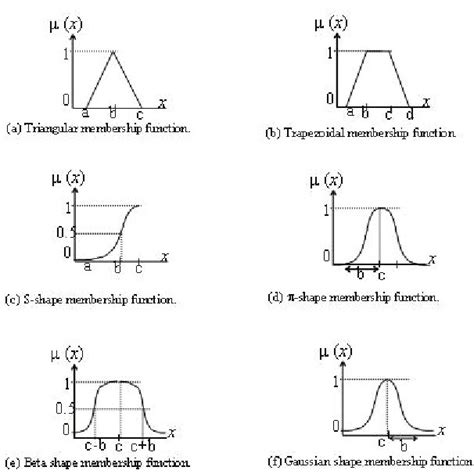
\includegraphics[draft=false,width=0.5\linewidth]{all}
        \caption{Типы функций принадлежности}
        \label{ris:image}
    \end{figure}
    Каждая из этих функций принадлежности имеет свои преимущества и недостатки, и выбор конкретной функции зависит от специфики задачи и данных. В данной работе будут рассмотрены треугольная функция принадлежности, Гауссова функция принадлежности и трапециевидная функция принадлежности, как наиболее популярные.

    \subsubsection{Алгоритмы дефаззификации}
    \textbf{Дефаззификация} - это процесс преобразования нечеткого вывода экспертной системы в точное числовое значение. Это необходимо для того, чтобы принять конкретное решение на основе нечеткого вывода. Существует несколько методов дефаззификации, рассмотрим некоторые из них.\\
    ~\\
    \textbf{Метод центра тяжести}\\
    Метод центра тяжести (COG) вычисляет центр тяжести функции принадлежности, используя следующую формулу:\\

    \[
        COG = \frac{\int x \cdot \mu(x) dx}{\int \mu(x) dx},
    \]
    - \(x\) - это точка на оси X,\\
    - \(\mu(x)\) - это степень принадлежности точки \(x\) к нечеткому множеству.\\

    В этой формуле числитель представляет собой интеграл от произведения каждой точки на оси X на ее степень принадлежности к нечеткому множеству. Знаменатель - это интеграл от степени принадлежности каждой точки на оси X к нечеткому множеству. Результатом является точка на оси X, которая представляет собой "{}центр тяжести"{} функции принадлежности.\\
    ~\\
    Этот метод обеспечивает хороший баланс между точностью и вычислительной сложностью, и он широко используется в различных приложениях, включая системы управления, прогнозирование и анализ данных.\\
    ~\\
    \textbf{Метод биссектрисы площади}\\
    Метод биссектрисы площади (Area Bisector method) или метод центра площади (Center of Area method) - это метод дефаззификации, который вычисляет центр тяжести под областью нечеткого множества. Этот метод предполагает, что каждая точка в области имеет одинаковую важность.Метод биссектрисы площади (Area Bisector method) или метод центра площади (Center of Area method) - это метод дефаззификации, который вычисляет центр тяжести под областью нечеткого множества. Этот метод предполагает, что каждая точка в области имеет одинаковую важность.\\
    ~\\
    Алгоритм дефаззификации методом биссектрисы площади можно описать следующим образом:\\
    ~\\
    1. Вычислить общую площадь под нечетким множеством. Это можно сделать, например, с помощью интегрирования.\\
    ~\\
    2. Найти точку, которая делит область под нечетким множеством на две равные части. Это можно сделать, например, с помощью метода бисекции.\\
    ~\\
    Формула для вычисления центра тяжести в методе биссектрисы площади выглядит следующим образом:\\
    ~\\
    \[
        COA = \frac{\int x \cdot \mu(x) dx}{\int \mu(x) dx},
    \]
    - \(COA\) - центр тяжести,\\
    - \(x\) - значение переменной,\\
    - \(\mu(x)\) - степень принадлежности значения \(x\) к нечеткому множеству.\\
    ~\\
    Этот метод дефаззификации обеспечивает хорошие результаты, когда форма нечеткого множества симметрична. Если форма нечеткого множества асимметрична, результат может быть искажен.\\
    ~\\
    \textbf{Метод среднего максимума}\\
    Метод среднего максимума вычисляет среднее значение всех максимальных значений функции принадлежности.\\
    ~\\
    Пусть $A$ - нечеткое множество, представленное своей функцией принадлежности $\mu_A(x)$ на универсальном множестве $X$. Тогда значение дефаззификации $x^*$ по методу среднего максимума определяется следующим образом:\\
    ~\\
    1. Найти все значения $x$, для которых $\mu_A(x)$ достигает своего максимального значения (назовем это множество $X_m$).\\
    2. Вычислить среднее значение всех элементов в $X_m$.\\
    ~\\
    В математической форме это можно записать так:\\
    ~\\
    $$x^* = \frac{1}{n} \sum_{x \in X_m} x,$$

    $n$ - количество элементов в $X_m$.\\
    ~\\
    Этот метод обычно используется, когда функция принадлежности имеет несколько максимумов. Он предоставляет более "{}сбалансированный"{} результат по сравнению с другими методами, такими как метод максимума (Maximum), который просто выбирает значение $x$, где функция принадлежности достигает своего максимума.
    ~\\
    \textbf{Метод максимума максимумов}\\
    Метод максимума максимумов выбирает среднее значение всех максимальных значений функции принадлежности. Этот метод обычно используется, когда функция принадлежности имеет несколько пиковых значений.

    Алгоритм MoM можно описать следующим образом:

    1. Найти все максимальные значения функции принадлежности. Это могут быть одно или несколько значений, в зависимости от формы функции принадлежности.

    2. Вычислить среднее значение всех найденных максимальных значений.

    Математически это можно выразить следующим образом:

    Пусть $A$ - нечеткое множество, представленное своей функцией принадлежности $μ_A(x)$, и пусть $X$ - множество всех $x$, для которых $μ_A(x)$ достигает своего максимального значения. Тогда центроид $C$ множества $X$ вычисляется по формуле:

    $$C = \frac{1}{|X|} \sum_{x \in X} x,$$

    $|X|$ - количество элементов в множестве $X$.

    Этот метод обеспечивает хорошие результаты, когда функция принадлежности имеет несколько пиков, но может быть неэффективным, если пики имеют различную высоту или ширину.
    ~\\
    \textbf{Метод минимума максимумов}\\
    Метод минимума максимумов работает следующим образом:

    1. Находятся все максимумы функции принадлежности нечеткого множества.
    2. Из этих максимумов выбирается минимальное значение.

    Математически это можно выразить следующим образом:

    Пусть $A$ - нечеткое множество, заданное своей функцией принадлежности $\mu_A(x)$ на некотором универсальном множестве $X$. Тогда центр тяжести $z$ вычисляется по формуле:

    $$z = \min_{x \in X} \max \mu_A(x)$$

    Этот метод обычно используется, когда необходимо найти наиболее консервативное значение, так как он выбирает наименьшее из максимальных значений. Однако, этот метод может быть неэффективным, если функция принадлежности имеет несколько пиков, так как он не учитывает их вклад в общее значение.
    ~\\
    В качестве алгоритмов дефаззификации были выбраны Метод центра тяжести и Метод среднего максимума как наиболее популярные.

    \subsubsection{Алгоритмы дефаззификации для выбранных типов нечетких множеств}
    В данном разделе рассматриваются алгоритмы дефаззификации для нечетких множеств 1 и 2 типа, а также для интуиционистских нечетких множеств. Дефаззификация является ключевым этапом в процессе использования нечетких множеств, поскольку позволяет перевести нечеткую информацию в точные числовые значения.

    \textbf{Нечеткие множества 1 типа}
    Нечеткие множества 1 типа характеризуются функцией принадлежности, которая принимает значения в интервале [0,1]. Один из популярных методов дефаззификации для таких множеств - метод центра тяжести (COG).

    \textbf{Метод центра тяжести}
    Метод центра тяжести определяется следующим образом:
    \[
        x^* = \frac{\int_{X} x \mu_A(x) \, dx}{\int_{X} \mu_A(x) \, dx}
    \]
    $x^*$ - дефаззифицированное значение, $\mu_A(x)$ - функция принадлежности нечеткого множества $A$, $X$ - универсум.

    \textbf{Нечеткие множества 2 типа}
    Нечеткие множества 2 типа включают функцию принадлежности, которая сама по себе является нечетким множеством. Для дефаззификации таких множеств часто используется метод расширенного центра тяжести.

    \textbf{Метод расширенного центра тяжести}
    Метод расширенного центра тяжести для нечетких множеств 2 типа можно выразить как:
    \[
        x^* = \frac{\int_{X} x \int_{J_x} \mu_{A}(x, u) \, du \, dx}{\int_{X} \int_{J_x} \mu_{A}(x, u) \, du \, dx}
    \]
    $J_x$ - интервал значений вторичной принадлежности при фиксированном $x$.

    \textbf{Интуиционистские нечеткие множества}
    Интуиционистские нечеткие множества характеризуются функциями степени принадлежности и степени непринадлежности. Дефаззификация таких множеств может быть выполнена с использованием индекса оптимизма\cite{litlink23}.

    \textbf{Индекс оптимизма}
    Индекс оптимизма определяется как:
    \[
        x^* = \frac{\int_{X} x (\mu_A(x) - \nu_A(x)) \, dx}{\int_{X} (\mu_A(x) - \nu_A(x)) \, dx}
    \]
    где $\mu_A(x)$ и $\nu_A(x)$ - степени принадлежности и непринадлежности соответственно.\\
    ~\\
    Описанные методы дефаззификации могут быть использованы в дальнейшем развитии работы, так как в рамках выпускной квалификационной работы реализация всех существующих методов не является первым приоритетом.
    \subsubsection {Схема расчета по шагам (reasoning process)}
    В данном разделе описывается алгоритм анализа нечетких когнитивных карт (НКК), используемый для моделирования восприятия факторов успеха IT-проектов. НКК позволяют анализировать и прогнозировать динамику системы на основе взаимодействия ее элементов.

    \textbf{Схема расчета по шагам для нечётких множеств первого типа}\\
    Для анализа НКК, использующих нечёткие множества первого типа, используется следующий алгоритм:

    \begin{tabbing}
        \hspace*{2em}\= \hspace*{2em}\= \hspace*{2em}\= \kill
        \textbf{Input:} $C, A, S_0, \alpha, \epsilon, maxIter$ \\
        \textbf{Output:} Final state vector $S$ \\
        1: \> $S \gets S_0$ \\
        2: \> $iter \gets 0$ \\
        3: \> \textbf{while} $iter < maxIter$ \textbf{do} \\
        4: \> \> $S_{new} \gets \textbf{zero}(n)$ \\
        5: \> \> \textbf{for} $i \gets 1$ \textbf{to} $n$ \textbf{do} \\
        6: \> \> \> $sum \gets 0$ \\
        7: \> \> \> \textbf{for} $j \gets 1$ \textbf{to} $n$ \textbf{do} \\
        8: \> \> \> \> $sum \gets sum + A[i, j] \cdot f(S[j])$ \\
        9: \> \> \> \textbf{end for} \\
        10: \> \> \> $S_{new}[i] \gets f(sum)$ \\
        11: \> \> \textbf{end for} \\
        12: \> \> \textbf{if} $\|S_{new} - S\| < \epsilon$ \textbf{then} \\
        13: \> \> \> \textbf{break} \\
        14: \> \> \textbf{end if} \\
        15: \> \> $S \gets \alpha \cdot S_{new} + (1 - \alpha) \cdot S$ \\
        16: \> \> $iter \gets iter + 1$ \\
        17: \> \textbf{end while} \\
        18: \> \textbf{return} $S$ \\
    \end{tabbing}
    Алгоритм представлен в псевдокоде, где $C$ - матрица факторов, $A$ - матрица весов связей, $S_0$ - начальное состояние системы, $\alpha$ - коэффициент сглаживания, $\epsilon$ - порог сходимости, $maxIter$ - максимальное количество итераций. Функция $f$ - функция активации.\\
    ~\\
    \textbf{Объяснение алгоритма}
    \begin{itemize}
        \item \textbf{Инициализация}: Начальное состояние $S_0$ задается вектором начальных значений факторов.
        \item \textbf{Итерационный процесс}: На каждом шаге вычисляется новое состояние системы $S_{new}$, используя текущее состояние $S$ и матрицу весов $A$.
        \item \textbf{Функция активации $f$}: Применяется к каждому элементу суммы взвешенных состояний, может быть линейной или нелинейной (например, сигмоид).
        \item \textbf{Критерий остановки}: Итерации продолжаются до тех пор, пока изменение состояния не станет меньше заданного порога $\epsilon$ или не будет достигнуто максимальное количество итераций $maxIter$.
        \item \textbf{Сглаживание}: Параметр $\alpha$ используется для сглаживания переходов между состояниями, чтобы избежать резких изменений.
    \end{itemize}
    Этот алгоритм позволяет анализировать динамику IT-проекта на основе взаимодействия различных факторов успеха, представленных в когнитивной карте, использующую нечёткие множества первого типа.

    \textbf{Схема расчета по шагам для нечётких множеств второго типа}\\
    Алгоритм анализа нечетких когнитивных карт для нечётких множеств второго типа можно представить следующим образом:

    \begin{tabbing}
        \hspace*{2em}\= \hspace*{2em}\= \hspace*{2em}\= \kill
        \textbf{Входные данные:} $C, A, S0, \alpha, \epsilon, maxIter$ \\
        \> \textbf{где:}\\
        \> $C$ \> -- матрица весов связей между концептами,\\
        \> $A$ \> -- начальные значения концептов,\\
        \> $S0$ \> -- начальное состояние карты,\\
        \> $\alpha$ \> -- коэффициент скорости обучения,\\
        \> $\epsilon$ \> -- порог сходимости,\\
        \> $maxIter$ \> \> -- максимальное число итераций.\\
        \textbf{Выходные данные:} $St$ -- состояние карты в момент времени $t$.\\
        \textbf{Метод:} \\
        \> \textbf{Шаг 1:} Инициализация $St = S0$.\\
        \> \textbf{Шаг 2:} \= Для $t = 1$ до $maxIter$ выполнить:\\
        \> \> \textbf{Шаг 2.1:} Рассчитать новое состояние каждого концепта $ci$:\\
        \> \> \> $S't(ci) = f\left(\sum{j} C{ij} \cdot G(S{t-1}(cj)) + (1 - \alpha) \cdot S{t-1}(ci)\right)$,\\
        \> \> \> \hspace*{1em} где $f$ -- функция активации, $G$ -- функция принадлежности нечеткого множества второго типа. \\
        \> \> \textbf{Шаг 2.2:} Обновление состояния: $St = S't$ \\
        \> \> \textbf{Шаг 2.3:} Проверка критерия остановки:\\
        \> \> \> Если $\|St - S{t-1}\| < \epsilon$, то выход. \\
        \textbf{Шаг 3:} \= Возврат $St$. \\
    \end{tabbing}

    Этот алгоритм начинается с инициализации состояния карты, осуществляет итеративные вычисления для обновления состояния каждого концепта на основе предыдущего состояния и весов матрицы $C$, а также функций нечеткости второго типа для каждого концепта. Процесс продолжается до тех пор, пока изменения состояний не станут меньше заданного порога $\epsilon$ или не будет достигнуто максимальное число итераций.
    ~\\
    \textbf{Объяснение алгоритма}\\
    Алгоритм использует систему взаимодействующих концептов, которые модифицируются на каждом шаге итерации с учетом весов связей и нечеткости второго типа. Система продолжает адаптироваться до достижения сходимости, определяемой порогом $\epsilon$, либо до исчерпания разрешенного числа итераций $maxIter$. Этот процесс позволяет картам отображать более сложные и неопределенные связи между концептами.\\
    ~\\
    \textbf{Схема расчета по шагам для интуиционистских нечетких множеств}\\
    Для анализа нечетких когнитивных карт (НКК) в рамках интуиционистских нечетких множеств (ИНМ), мы можем использовать следующий алгоритм. Нечеткие когнитивные карты могут быть полезны для моделирования и анализа поведения систем, когда учитывается неполнота и неопределенность знаний. ИНМ добавляют дополнительный уровень, позволяя одновременно учитывать степень принадлежности и не принадлежности элемента.\\
    ~\\
    Шаг 1: Определение ИНМ\\
    Для каждого концепта $C_i$ в НКК определим интуиционистское нечеткое множество $A_i$, где каждый элемент $x \in X$ (пространство элементов) характеризуется степенями принадлежности $\mu_{A_i}(x)$ и непринадлежности $\nu_{A_i}(x)$ так, что $\mu_{A_i}(x) + \nu_{A_i}(x) \leq 1$ для всех $x \in X$.\\

    $$A_i(x) = \{\mu_{A_i}(x), \nu_{A_i}(x)\}$$
    ~\\
    Шаг 2: Матрица влияний\\
    Создаем матрицу влияний $W$ размерности $n \times n$, где $n$ — количество концептов в НКК. Элемент $w_{ij}$ матрицы $W$ описывает влияние концепта $C_j$ на концепт $C_i$. Влияние может быть как положительным, так и отрицательным.\\

    $$W = [w_{ij}]_{n \times n}$$
    ~\\
    Шаг 3: Расчет новых значений концептов\\
    Используем правила активации для обновления степеней принадлежности и непринадлежности для каждого концепта. Вычисление нового состояния концептов $A_i^n$ происходит на основе предыдущих состояний $A_i^{n-1}$ и влияния других концептов в соответствии с матрицей $W$.\\

    $$\mu_{A_i^n}(x) = f\left(\sum_{j=1}^n w_{ij} \cdot \mu_{A_j^{n-1}}(x)\right)$$
    $$\nu_{A_i^n}(x) = g\left(\sum_{j=1}^n w_{ij} \cdot \nu_{A_j^{n-1}}(x)\right)$$
    где $f$ и $g$ — функции активации, выбираемые в зависимости от характера влияния и типа концептов.\\
    ~\\
    Шаг 4: Критерии сходимости\\
    Алгоритм повторяется, пока не будет достигнут критерий сходимости, например, когда изменения степеней принадлежности и непринадлежности для всех концептов становятся ниже заданного порогового значения.\\
    ~\\
    Шаг 5: Интерпретация результатов\\
    По завершении алгоритма анализируем полученные значения ИНМ для каждого концепта, что позволяет сделать выводы о стабильности системы, влиянии определенных концептов и возможных сценариях развития.\\
    ~\\
    Этот алгоритм представляет собой один из подходов к анализу НКК с использованием ИНМ и может быть адаптирован или дополнен в зависимости от специфики задачи и данных.\\
    \subsection {Описание входных и выходных данных программы}

    \subsubsection{Входные данные}
    Входными данными для программы являются пользовательские наборы факторов успеха IT-проекта и связей между ними. Фактор является представлением определенной особенности или аспекта IT-проекта, который может влиять на его успех. Связи между факторами представляют собой отношения между ними в формальной или относительной форме.\\
    ~\\
    Однако, стоит отметить, что факторы успеха IT-проекта необязательно являются входными параметрами в готовом виде. Они могут формироваться в процессе обсуждения проекта со стейкхолдерами и являются результатом командной работы нескольких человек.\\
    ~\\
    Каждый фактор успеха определяется оператором и представляет собой идентификатор и соответствующее ему имя. При добавлении факторов оператор может выбрать из списка популярных факторов, а также добавить собственный.\\
    ~\\
    Связи между факторами определяются оператором с помощью выбора двух добавленных факторов и указания степени влияния. Они представляют собой кортеж из трех элементов: исходного фактора, конечного фактора и веса связи в неформальном виде.\\
    ~\\
    Факторы и связи между ними задаются оператором в интуитивно понятном интерфейсе.

    \subsubsection{Выходные данные}
    Программа предоставляет следующие выходные данные:\\
    \begin{enumerate}
        \item  Когнитивная Карта: Программа выдает когнитивную карту, которая иллюстрирует влияние различных факторов на успех IT-проекта. Эта карта включает в себя узлы, представляющие факторы, и связи между ними, показывающие степень влияния этих факторов друг на друга.
        \item  Визуализация Карты: Программа обеспечивает средства для визуализации этой карты, позволяющие оператору и стейкхолдерам лучше понять, как факторы связаны друг с другом.
        \item  Анализ Сценариев: Программа может выполнять анализ сценариев, изменяя наличие или влияние отдельных факторов, чтобы помочь оператору предсказать, как изменения в этих факторах могут повлиять на итоговый успех IT-проекта через влияние на другие факторы модели.
        \item  Результаты Моделирования: Программа выдает итоговые результаты моделирования, демонстируя, как изменения в отдельных факторах или их комбинации могут влиять на успех IT-проекта. Это также может включать кумулятивное впечатление от всех факторов, отражающее общее состояние успешности проекта.
        \item  Экспорт Данных: Программа обеспечивает возможность экспорта выходных данных для дальнейшего анализа, отчетности или представления результатов третьим лицам. Это может быть выполнено в различных форматах, таких как CSV, PDF или HTML.
    \end{enumerate}
    Результаты моделирования представляют собой совокупность данных, которые требуют детального анализа и интерпретации. Это процесс, который включает в себя активное участие всех участников проекта, включая стейкхолдеров. Результаты моделирования, преобразованные в словесную форму, становятся основой для дальнейшего обсуждения, анализа и формирования окончательных выводов.\\
    \subsection {Интерфейс программы}
    Интерфейс программы включает в себя панель инструментов и область визуализации когнитивной карты.\\
    ~\\
    Панель инструментов включает в себя поля ввода для добавления факторов успеха и соответствующих связей, а также кнопки для добавления, изменения и удаления факторов и связей. оператору доступен функционал перемещения факторов на области визуализации нечеткой когнитивной карты для создания более удобного и наглядного расположения факторов.\\
    ~\\
    Область визуализации карты представляет собой интерактивное поле, на котором отображаются факторы и связи между ними. При добавлении фактора или связи в панели инструментов, они автоматически появляются на карте, предоставляя оператору непосредственную обратную связь.\\
    ~\\
    Связи между факторами подсвечиваются разными цветами в зависимости от степени связи, облегчая интерпретацию взаимного влияния факторов.\\
    ~\\
    Щелчок мыши по связи приводит к появлянию окна, в котором можно редактировать детали (характеристики) связи. Аналогично, щелчок мыши по фактору вызывает окно с редактированием характеристик выбранного фактора.\\
    ~\\
    Кнопка "{}Проанализировать карту"{} запускает алгоритм анализа карты. При этом оператор имеет возможность указать число шагов, которые должен произвести алгоритм. В любой момент выполнения алгоритма анализа оператор может остановить его работу посредством кнопки "{}Стоп"{}.\\
    ~\\
    Также оператору доступно скачивание полученной картины в форматах PNG или SVG, что облегчает дальнейшую работу с результатами моделирования.\\
    ~\\
    Все элементы интерфейса разработаны в унифицированном стиле, обеспечивая удобное и интуитивно понятное взаимодействие с программой.\\
    \subsection {Выбор технических и программных средств}
    При проектировании и разработке программного обеспечения для моделирования восприятия факторов успеха IT-проекта с использованием нечетких когнитивных карт был осуществлен выбор следующих ключевых технических и программных средств:\\
    \begin{enumerate}
        \item Django. Django является мощным и гибким веб-фреймворком на Python, который позволяет быстро создавать сложные веб-приложения. Он обеспечивает высокий уровень безопасности и поддерживает разработку на основе модели данных, что значительно ускоряет процесс создания приложения. Django также содержит сложные инструменты для обработки форм и аутентификации пользователей.
        \item JavaScript. Этот язык программирования используется для создания клиентской части веб-приложения. Он обеспечивает интерактивность и динамичность интерфейса пользователя, позволяет обрабатывать пользовательский ввод, управлять элементами страницы и взаимодействовать с сервером.
        \item Дополнительные средства. Для работы с базами данных может быть выбрана реляционная база данных Postgres, которая обеспечивает достаточный функционал для хранения и обработки данных в данном проекте.
    \end{enumerate}
    Все выбранные технологии являются открытыми и широко используются в практической деятельности, что обеспечивает хорошую информационную поддержку и возможности для дальнейшего развития проекта.

    \newpage
    \section {Ожидаемые технико-экономические показатели}
    \subsection {Предполагаемая потребность}
    Программа для моделирования восприятия факторов успеха IT-проекта с использованием нечетких когнитивных карт предназначена для обеспечения качественного и объективного анализа ключевых факторов, определяющих успех реализации IT-проекта.

    \subsubsection{Организации и ИТ-отделы}
    Основными потребителями программы могут стать ИТ-отделы различных организаций. Программа позволит учет влияния различных факторов на итоговый успех проекта, таких как качество руководства проектом, навыки и опыт команды, используемые технологии и методологии, соответствие требованиям заказчика и т.д.

    \subsubsection{Исследовательские центры и учебные учреждения}
    В учебных целях программа может использоваться в исследовательских центрах и вузах для изучения принципов моделирования и анализа факторов успеха в IT-проектах.

    \subsubsection{IT-консалтинг и аналитические компании}
    Аналитические компании и IT-консалтинговые агентства могут использовать программу для предоставления услуг по оценке и прогнозированию успешности IT-проектов на основе моделирования взаимосвязи факторов успеха.\\
    ~\\
    Таким образом, данная программа позволяет не только получить количественное и качественное представление о будущем успехе проекта, но и выявить основные пути оптимизации ресурсов и рисков.\\
    ~\\
    Однако, следует отметить, что окончательные выводы и интерпретация полученных данных — это результат коллективной работы и обсуждения в группе. Моделирование предоставляет нам возможность преобразовать сложные процессы в понятные и интерпретируемые данные. Эти данные, в свою очередь, конвертируются в слова, которые мы используем для общения с заинтересованными сторонами. Это обеспечивает продолжение диалога, позволяет формировать выводы и принимать обоснованные решения.\\
    \subsection {Первоначальная оценка успеха проекта}
    Первоначальная оценка успеха разработанной программы для моделирования восприятия факторов успеха IТ-проекта с использованием нечетких когнитивных карт проведена по следующим критериям:
    \begin{enumerate}
        \item \textbf{Соответствие заявленному техническому заданию:} Разработанная программа должна полностью соответствовать требованиям и функционалу, описанным в техническом задании. Должна быть проработана каждая деталь, начиная от общей концепции и заканчивая отдельными элементами интерфейса.
        \item \textbf{Качество документации:} К программе должна прилагаться подробная и понятная документация, которая позволит оператору без проблем воспользоваться всеми функциями программы. Документация должна отражать все аспекты использования программы, включая описание возможных ошибок и способов их решения.
        \item \textbf{Удобство использования:} Программа должна быть удобной в использовании. Интерфейс должен быть интуитивно понятным, а возможности программы - легко доступными.
        \item \textbf{Стабильность работы:} Программа должна работать стабильно и без сбоев, вне зависимости от объема обрабатываемых данных и сложности задач.
    \end{enumerate}
    По результатам оценки по вышеуказанным критериям можно судить о первоначальном успехе проекта. При наличии значимых недостатков и отклонений от требований ТЗ должна быть проведена доработка программы и устранить выявленные проблемы.
        \subsection {Последующая оценка успеха проекта}
    Последующая оценка успеха проекта проводится по следующим критериям:
    \begin{enumerate}
        \item \textbf{Решение комиссии о дипломной работе:} Оценка комиссии является непосредственным показателем успеха проекта. Комиссия будет изучать все аспекты работы, начиная от проработанности задания до его выполнения.

        \item \textbf{Полученная оценка:} Конечная оценка на дипломную работу — важный показатель, но не единственный. Она является отражением всех сильных и слабых сторон дипломной работы, которые были замечены в ходе ее защиты.

        \item \textbf{Комментарии и оценка руководителя работы:} Научный руководитель оценивает работу как научное исследование и анализирует ее на основе его понимания предметной области и опыта проведения исследований.
    \end{enumerate}
    \subsection {Конечный параметр оценки успеха проекта}
    Для оценки успеха IT-проекта необходимы точные и конкретные параметры оценки. В контексте нашего проекта, главными параметрами оценки будут:
    \begin{itemize}
        \item \textbf{Количество пользователей}: Этот параметр отражает общее количество пользователей, использующих данную программу. Увеличение этого числа указывает на успех программы на рынке.
        \item \textbf{Оценки пользователей}: Оценки и отзывы от пользователей могут дать ценную информацию о том, насколько хорошо программа отвечает на потребности пользователей, и каких улучшений она требует.
        \item \textbf{Количество упоминаний в исследовательских работах}: Чем больше программа упоминается в академических или промышленных исследованиях, тем больше у неё влияние на сферу науки и технологии, что является признаком её успеха.
        \item \textbf{Популярность в интернете}: Этот параметр можно измерить через различные индикаторы, такие как количество поисковых запросов, упоминаний в социальных сетях и т.д. Повышение этого показателя говорит о том, что программа привлекает все больше и больше интереса.
    \end{itemize}
    Эти параметры являются совокупным показателем успеха данного проекта и будут использоваться для оценки и анализа эффективности продукта на протяжении всего его жизненного цикла.\\
    ~\\
    Дополнительно параметрами оценки успеха проекта являются параметры, которые могут быть выяснены только с помощью сбора метрик и получения обратной связи от пользователей:
    \begin{itemize}
        \item \textbf{Точность моделирования:} Итоговый продукт должен обеспечивать точное моделирование восприятия IT-проектов, при этом обеспечивая возможность легко включать или исключать различные параметры.
        \item \textbf{Эффективность использования:} Использование программы не должно требовать значительных затрат времени или ресурсов для погружения в детали использования программы.
        \item \textbf{Адаптивность к изменениям:} Программа должна быть способна адаптироваться к изменению условий или параметров внешней среды.
        \item \textbf{Удобство интерфейса:} Интерфейс программы должен быть интуитивно понятен для пользователей, обеспечивая легкий доступ к основным функциям и настройкам.
        \item \textbf{Возможность масштабирования:} Программа должна предоставлять возможность масштабирования для работы с более крупными или сложными проектами в будущем.
    \end{itemize}
    Успех проекта будет определен по достижению этих целей и учету обратной связи от пользователей для дальнейших усовершенствований. Дополнительные параметры могут быть выявлены в ходе общения со стейкхолдерами и потенциальными пользователями.
    \subsection {Экономические преимущества разработки по сравнению с отечественными и зарубежными аналогами}
    В сравнении с отечественными и зарубежными аналогами, разрабатываемое программное обеспечение обладает рядом значительных экономических преимуществ. Прежде всего, оно предоставляется оператору бесплатно, тем самым исключая необходимость трат на его приобретение. В качестве веб-приложения, оно не требует дополнительного внедрения и поддержки, что существенно снижает затраты на эксплуатацию.\\
    ~\\
    Кроме того, на данный момент на рынке не представлено программ, специально ориентированных на моделирование восприятия IT-проектов с использованием нечетких когнитивных карт. Данное программное обеспечение является специализированным инструментом в этой области, что повышает его ценность для IT-компаний, команд разработчиков и людей, использующих программу в образовательных целях.\\
    ~\\
    Таким образом, использование данного ПО позволяет оптимизировать расходы, связанные с прогнозированием успеха IT-проектов, а также повысить точность и оперативность соответствующих аналитических работ.

    \newpage
    \section{Заключение}
    \subsection{Итоги анализа литературы}
    Анализ литературы показал, что успешное выполнение IT-проектов становится всё более важным для организаций различных сфер деятельности из-за растущей зависимости бизнеса от технологий. Однако измерение и предсказание успеха IT-проектов остаётся сложной задачей, требующей учёта множества факторов, характеризуемых неопределённостью и взаимосвязью.\\
    ~\\
    Программа для моделирования восприятия факторов успеха IT-проектов с использованием нечетких когнитивных карт является актуальной из-за способности данных карт моделировать нечетко определённые и интерпретируемые факторы. Методология когнитивного моделирования, предложенная Робертом Аксельродом и усовершенствованная нечеткими когнитивными картами Барта Коско, повторно привлекает внимание исследователей для решения задач в условиях неопределённости.\\
    ~\\
    В последние годы проводятся многочисленные исследования по применению нечетких когнитивных карт в различных областях, включая IT-проекты. Их применение позволяет моделировать сложные взаимосвязи и получать результаты на основе неопределённой информации. У нечетких когнитивных карт есть преимущества, такие как удобство визуализации сложных идей и информации, улучшение понимания и организации знаний, а также содействие эффективному принятию решений.\\
    ~\\
    Тем не менее, существуют и недостатки использования данных карт: сложность создания и интерпретации при большом объёме информации и сложных взаимосвязях, а также субъективность из-за зависимости от знаний и восприятия отдельных людей или групп.\\
    ~\\
    Во всех рассмотренных работах подчеркивается важность определения и оценки критических факторов успеха (CSF) для IT-проектов, что подтверждает актуальность выбранной темы исследования.\\
    ~\\
    Таким образом, разработка программы для моделирования восприятия факторов успеха IT-проектов с использованием нечетких когнитивных карт является актуальным и полезным подходом для решения сложной проблемы IT-управления и планирования.\\
    \subsection{Результаты разработки веб-приложения}

    В рамках данной дипломной работы было разработано веб-приложение с использованием фреймворка Django. Приложение предназначено для моделирования факторов успеха IT-проектов с помощью нечетких когнитивных карт.

    Основные функции веб-приложения включают:
    \begin{itemize}
        \item Регистрация и авторизация пользователей.
        \item Управление проектами: пользователи могут создавать, редактировать и удалять свои проекты.
        \item Моделирование факторов успеха проекта с использованием когнитивной карты. Для визуализации карты и взаимодействия с ней была использована библиотека d3.js.
        \item Запуск процесса анализа (reasoning process) созданной когнитивной карты.
        \item Предоставление подробного отчёта о результатах работы алгоритма. Данный отчёт может быть использован пользователем для дальнейшего обсуждения с заинтересованными сторонами (стейкхолдерами).
    \end{itemize}

    \subsubsection{Регистрация и авторизация пользователей}

    Система регистрации и авторизации позволяет пользователям создавать уникальные учётные записи, благодаря которым они могут получить доступ к своим проектам. В процессе регистрации пользователь вводит основные персональные данные и создаёт пароль для учётной записи. После успешной регистрации пользователь может авторизоваться в системе с использованием введённых параметров.

    \subsubsection{Управление проектами}

    Каждый зарегистрированный пользователь имеет возможность создавать новые проекты, редактировать существующие и удалять их. Эта функция позволяет пользователям вести учёт своих IT-проектов и управление ими внутри веб-приложения.

    \subsubsection{Моделирование факторов успеха проекта}

    Центральной функцией веб-приложения является моделирование факторов успеха IT-проекта с помощью когнитивной карты. Для этого была использована библиотека d3.js, которая обеспечивает интерактивную визуализацию когнитивной карты. Пользователь может добавлять и связывать факторы на карте, создавая модель успеха проекта.

    \subsubsection{Запуск анализа НКК}

    После создания и настройки когнитивной карты, пользователь может запустить алгоритм анализа НКК (reasoning process). Этот процесс анализирует созданную модель и вычисляет результаты на основе введённых данных и связей между факторами.

    \subsubsection{Отчёт о результатах работы алгоритма}

    Программа предоставляет подробный отчёт о результатах работы алгоритма, который включает:
    \begin{itemize}
        \item \textbf{Матрица весов факторов:} Отражает степень влияния одного фактора на другой. Помогает понять, какие факторы имеют наибольшее влияние на успех проекта.
        \item \textbf{Анализ критических факторов успеха (CSF):} Идентифицирует наиболее значимые факторы, влияющие на успех проекта, позволяя концентрировать усилия на этих аспектах.
        \item \textbf{Влияние отдельных факторов:} Оценивает влияние каждого фактора на общий успех проекта, помогая определить, какие факторы нуждаются в усилении или изменении.
        \item \textbf{Итерационные вычисления:} Отображает процесс итеративных вычислений, показывающий изменения в системе при изменении одного из факторов и симулирующий различные сценарии.
        \item \textbf{Конвергенция карты:} Уровень стабилизации модели после нескольких итераций, показывающий, насколько система приближается к равновесию и оценивающий устойчивость предложенной модели.
    \end{itemize}

    Этот отчёт может быть использован при дальнейшем обсуждении результатов со стейкхолдерами, что способствует более эффективному управлению и планированию IT-проектов.\\
    ~\\
    Таким образом, разработанное веб-приложение предоставляет пользователям инструмент для моделирования и анализа факторов успеха IT-проектов, что подтверждает его полезность и актуальность для решения поставленных задач.\\
    \subsection{Проведение тестирования программы}

    Для обеспечения качества работы разработанного веб-приложения и подтверждения его функциональности было проведено тестирование программы. Тестирование включало несколько этапов, каждый из которых был направлен на проверку различных аспектов системы.

    \subsubsection{Методика проведения тестирования}

    Тестирование проводилось с использованием методик функционального и пользовательского тестирования. Основное внимание уделялось следующим аспектам:
    \begin{itemize}
        \item \textbf{Функциональность:} Проверка корректной работы всех основных функций приложения, включая регистрацию и авторизацию пользователей, управление проектами, моделирование факторов успеха и запуск процесса рассуждения.
        \item \textbf{Usability:} Оценка удобства использования интерфейса приложения для пользователей, не обладающих глубокими техническими знаниями.
        \item \textbf{Производительность:} Измерение времени отклика и производительности приложения при обработке большого объема данных и сложных когнитивных карт.
        \item \textbf{Надежность:} Проверка устойчивости приложения при различных сценариях использования, включая крайние и нестандартные случаи.
    \end{itemize}

    \subsubsection{Результаты тестирования}

    \paragraph{Функциональность:}
    Все основные функции веб-приложения были протестированы и показали корректную работу. В частности:
    \begin{itemize}
        \item Регистрация и авторизация пользователей прошли успешно, без возникновения ошибок.
        \item Управление проектами (создание, редактирование и удаление) функционировало корректно.
        \item Моделирование факторов успеха с использованием когнитивной карты работало стабильно, были проверены различные сценарии создания и редактирования карт.
        \item Запуск процесса рассуждения показал корректные результаты анализа на основе введённых данных.
    \end{itemize}

    \paragraph{Usability:}
    Интерфейс приложения был оценён тестовой группой пользователей. Получены положительные отзывы о простоте и интуитивности интерфейса. Основные улучшения, предложенные пользователями, были направлены на увеличение информативности сообщений и подсказок.

    \paragraph{Производительность:}
    Тестирование производительности показало, что приложение стабильно работает при обработке когнитивных карт средней сложности. В отдельных тестах обработка больших и сложных карт требовала увеличенного времени вычислений, что может быть улучшено в будущих версиях приложения.

    \paragraph{Надежность:}
    Программа показала устойчивую работу при различных сценариях использования, включая стресс-тестирование и ввод некорректных данных. Были выявлены и устранены незначительные ошибки, связанные с обработкой исключений.

    \subsubsection{Выводы по результатам тестирования}

    Тестирование показало, что разработанное веб-приложение соответствует поставленным требованиям и успешно выполняет все заявленные функции. Основные аспекты системы, такие как функциональность, юзабилити, производительность и надежность, были проверены и подтвердили свою работоспособность. В будущем планируется дальнейшее тестирование и оптимизация для повышения производительности и удобства использования.

    \subsection{Использование результатов программы стейкхолдерами}

    Разработанное веб-приложение предоставляет пользователям ценную информацию о факторах, влияющих на успех IT-проектов. Важно подчеркнуть, что программа не делает самостоятельных выводов, а лишь предоставляет значения и результаты анализа. Конечное решение всегда остаётся за стейкхолдерами, которые интерпретируют данные и принимают управленческие решения на основе представленных результатов. Ниже описаны этапы и рекомендации, которые помогут стейкхолдерам более эффективно использовать результаты программы.

    \subsubsection{Этапы использования результатов программы}

    \begin{itemize}
        \item \textbf{Получение результатов анализа:}
        После моделирования факторов успеха с использованием нечеткой когнитивной карты и запуска процесса рассуждения пользователю предоставляется подробный отчет о результатах анализа. Этот отчет включает в себя матрицу весов факторов, критические факторы успеха, влияние отдельных факторов, итерационные вычисления и графическую визуализацию.
        \item \textbf{Первичный анализ результатов:}
        Стейкхолдеры проводит первичный анализ предоставленных данных, обращая особое внимание на критические факторы успеха и взаимосвязи между ними. Это позволяет выявить ключевые аспекты, требующие внимания.
        \item \textbf{Обсуждение результатов:}
        После первичного анализа стейкхолдеры должны провести обсуждение результатов. Это обеспечивает всесторонний обзор представленных данных и совместное понимание выявленных факторов и их взаимосвязей.
    \end{itemize}

    \subsubsection{Рекомендации по интерпретации результатов}

    \begin{itemize}
        \item \textbf{Погружение в контекст:}
        Прежде чем начать интерпретацию результатов, стейкхолдерам следует погрузиться в контекст проекта, чтобы лучше понимать характеристики каждой переменной и ее роль в проекте. Это поможет избежать неверной интерпретации значений.
        \item \textbf{Использование визуализаций:}
        Графическая визуализация нечеткой когнитивной карты помогает наглядно представить взаимосвязи между факторами. Стейкхолдеры должны обратить внимание на узлы с наибольшими весами и их связи, что поможет в выявлении критических точек.
        \item \textbf{Обсуждение сценариев:}
        Совместное обсуждение различных сценариев с участием всех заинтересованных сторон помогает понять, как изменения в одном факторе могут повлиять на общий успех проекта. Это способствует лучшему пониманию и подготовке к возможным рискам.
        \item \textbf{Экспертное мнение:}
        Привлечение экспертов для интерпретации сложных взаимосвязей и анализа предоставленных данных поможет получить более точные и обоснованные выводы.
        \item \textbf{Дополнительные анализы:}
        Использование других методов анализа и инструментов, таких как SWOT-анализ или PEST-анализ, может дополнительно подтвердить или опровергнуть результаты, предоставленные программой.
    \end{itemize}

    Таким образом, использование разработанного веб-приложения и интерпретация его результатов требует совместной работы стейкхолдеров и экспертов. Программа предоставляет ценную информацию, которая может служить основой для дальнейших управленческих решений. Важно помнить, что конечные выводы и действия должны основываться на совокупности представленных данных и экспертного мнения, чтобы обеспечить успех IT-проекта.

    \subsection{Перспективы будущих исследований}

    Разработка веб-приложения для моделирования восприятия факторов успеха IT-проектов с использованием нечетких когнитивных карт предоставляет множество возможностей для дальнейшего улучшения и расширения функционала. В частности, возможны следующие направления для дальнейших исследований и разработок:

    \begin{itemize}
        \item \textbf{Использование других типов нечетких множеств:}
        В текущей версии приложения используются нечеткие множества первого и второго типов, а также интуиционистские нечеткие множества. Однако, можно рассмотреть возможность внедрения дополнительных типов нечетких множеств, таких как нейрософские и многозначные нечеткие множества, которые могут предоставить новые перспективы в моделировании факторов успеха.

        \item \textbf{Применение других алгоритмов дефаззификации:}
        На данный момент используются метод центра тяжести, метод биссектрисы площади и метод среднего максимума для процесса дефаззификации. В дальнейшем можно рассмотреть применение других методов, таких как метод максимального вероятного значения, метод взвешенного среднего и метод минимального расстояния, что может улучшить точность и эффективность модели.

        \item \textbf{Использование других типов функций принадлежности:}
        В текущей версии приложения для параметризации используются треугольные, гауссовые и трапециевидные функции принадлежности. В будущем можно рассмотреть использование сложных функций принадлежности, таких как колоколоподобные функции, синусоидальные функции и функции с размытой границей, что может улучшить точность представления нечетких данных.

        \item \textbf{Увеличение количества лингвистических термов:}
        В настоящее время количество значений параметров ограничено небольшим числом. Увеличение числа лингвистических термов позволит более точно описывать нечеткие множества и улучшит моделирование сложных систем, позволяя вводить более разнообразные и точные оценки факторов успеха.

        \item \textbf{Упрощение ввода параметров для оператора:}
        На данный момент оператору необходимы минимальные знания теории нечетких множеств для ввода коэффициента сглаживания, порога сходимости и максимального количества итераций. В дальнейшем планируется упростить пользовательский интерфейс и повысить его интуитивность, что позволит упростить ввод параметров и сделать систему более доступной для пользователей без глубоких знаний в области теории нечетких множеств.
    \end{itemize}

    Эти направления дальнейшей работы позволят улучшить функциональность и точность разработанного веб-приложения, а также расширить его сферу применения, делая его более универсальным и удобным инструментом для моделирования факторов успеха IT-проектов.

    \subsection{Выводы}
    В результате проведенной работы была разработана и протестирована программа для моделирования факторов успеха IT-проектов с использованием нечетких когнитивных карт. Основные итоги приведены ниже.

    \begin{itemize}
        \item \textbf{Эффективность нечетких когнитивных карт:} Нечеткие когнитивные карты показали себя как эффективный инструмент для моделирования и анализа факторов успеха IT-проектов. Они позволяют визуализировать сложные взаимосвязи между факторами и учитывать их нечеткую природу.
        \item \textbf{Функциональность веб-приложения:} Разработанное веб-приложение успешно выполняет основные функции, такие как регистрация и авторизация пользователей, управление проектами, моделирование факторов успеха и запуск процесса рассуждения. Программа предоставляет пользователю подробный отчет о результатах работы алгоритма.
        \item \textbf{Удобство использования:} Интуитивный интерфейс и подробные руководство пользователя позволяют использовать приложение даже пользователям без глубоких знаний теории нечетких множеств.
        \item \textbf{Производительность и надежность:} Программа показала стабильную работу при различных сценариях использования, включая стресс-тестирование. Производительность системы удовлетворительна при обработке когнитивных карт средней сложности.
    \end{itemize}

    Таким образом, разработанное веб-приложение для моделирования факторов успеха IT-проектов с использованием нечетких когнитивных карт представляет собой эффективный и интуитивно понятный инструмент, способный существенно улучшить процессы планирования и управления IT-проектами в условиях неопределенности.

    \newpage
    \section{Список использованных источников}
    \begin{thebibliography}{}
        \bibitem{litlink1} ГОСТ 19.101-77. Единая система программной документации. Термины и определения: утвержден и введен в действие Постановлением Государственного комитета стандартов Совета Министров СССР от 20 мая 1977 г. № 1268 срок введения: с 01.01.1980 г. – URL: https://www.swrit.ru/doc/espd/19.001-77.pdf (дата обращения: 01.12.2023). – Текст: электронный.
        \bibitem{litlink2} ГОСТ 19.102-77. Единая система программной документации. Термины и определения: утвержден и введен в действие Постановлением Государственного комитета стандартов Совета Министров СССР от 20 мая 1977 г. № 1268 срок введения: с 01.01.1980 г. – URL: https://www.swrit.ru/doc/espd/19.102-77.pdf (дата обращения: 01.12.2023). – Текст: электронный.
        \bibitem{litlink3} 19.103-77. Единая система программной документации. Термины и определения: утвержден и введен в действие Постановлением Государственного комитета стандартов Совета Министров СССР от 20 мая 1977 г. № 1268 срок введения: с 01.01.1980 г. – URL: https://www.swrit.ru/doc/espd/19.103-77.pdf (дата обращения: 01.12.2023). – Текст: электронный.
        \bibitem{litlink4} ГОСТ 19.104-78. Единая система программной документации. Термины и определения: утвержден и введен в действие Постановлением Государственного комитета стандартов Совета Министров СССР от 20 мая 1977 г. № 1268 срок введения: с 01.01.1980 г. – URL: https://www.swrit.ru/doc/espd/19.104-78.pdf (дата обращения: 01.12.2023). – Текст: электронный.
        \bibitem{litlink5} ГОСТ 19.105-78. Единая система программной документации. Термины и определения: утвержден и введен в действие Постановлением Государственного комитета стандартов Совета Министров СССР от 20 мая 1977 г. № 1268 срок введения: с 01.01.1980 г. – URL: https://www.swrit.ru/doc/espd/19.105-78.pdf (дата обращения: 01.12.2023). – Текст: электронный.
        \bibitem{litlink6} ГОСТ 19.106-78. Единая система программной документации. Термины и определения: утвержден и введен в действие Постановлением Государственного комитета стандартов Совета Министров СССР от 20 мая 1977 г. № 1268 срок введения: с 01.01.1980 г. – URL: https://www.swrit.ru/doc/espd/19.106-78.pdf (дата обращения: 01.12.2023). – Текст: электронный.
        \bibitem{litlink7} ГОСТ 19.404-79. Единая система программной документации. Термины и определения: утвержден и введен в действие Постановлением Государственного комитета стандартов Совета Министров СССР от 20 мая 1977 г. № 1268 срок введения: с 01.01.1980 г. – URL: https://www.swrit.ru/doc/espd/19.404-79.pdf (дата обращения: 01.12.2023). – Текст: электронный.
        \bibitem{litlink8} ГОСТ 19.603-78. Единая система программной документации. Термины и определения: утвержден и введен в действие Постановлением Государственного комитета стандартов Совета Министров СССР от 20 мая 1977 г. № 1268 срок введения: с 01.01.1980 г. – URL: https://www.swrit.ru/doc/espd/19.603-78.pdf (дата обращения: 01.12.2023). – Текст: электронный.
        \bibitem{litlink9} ГОСТ 19.404-79. Единая система программной документации. Термины и определения: утвержден и введен в действие Постановлением Государственного комитета стандартов Совета Министров СССР от 20 мая 1977 г. № 1268 срок введения: с 01.01.1980 г. – URL: https://www.swrit.ru/doc/espd/19.404-79.pdf (дата обращения: 01.12.2023). – Текст: электронный.

        \bibitem{litlink10} \textit{Учебный офис ФКН ПИ} (2023) СПРАВОЧНИК УЧЕБНОГО ПРОЦЕССА НИУ ВШЭ. Выпускная квалификационная работа (ВКР) // Сайт hse.ru (https://www.hse.ru/studyspravka/vkr) Просмотрено: 30.11.2023.
        \bibitem{litlink11} \textit{Жернова Мария Олеговна} (2023) Учебные планы 2020 года набора // Сайт hse.ru (https://www.hse.ru/ba/se/learn\_plans) Просмотрено: 12.12.2023.

        \bibitem{litlink12} \textit{Robert Axelrod} (1976) Structure of Decision: The Cognitive Maps of Political Elites // Сайт jstor.org (https://www.jstor.org/stable/j.ctt13x0vw3) Просмотрено: 17 января 2024.
        \bibitem{litlink13} \textit{Bart Kosko} (1985) Fuzzy cognitive maps // Сайт sipi.usc.edu (http://sipi.usc.edu/~kosko/FCM.pdf) Просмотрено: 17 января 2024.
        \bibitem{litlink14} \textit{Papageorgiou, Elpiniki \& Papageorgiou, Konstantinos \& Dikopoulou, Zoumpoulia \& Mourhir, Asmaa} (2018) A Fuzzy Cognitive Map web-based tool for modeling and decision making // Сайт researchgate.net (https://www.researchgate.net/publication/336591466\_A\_Fuzzy\_Cognitive\_Map\_web-based\_tool\_for\_modeling\_and\_decision\_making) Просмотрено: 17.01.2024.
        \bibitem{litlink15} \textit{Felix Benjamín, Gerardo \& Nápoles, Gonzalo \& Falcon, Rafael \& Froelich, Wojciech \& Vanhoof, Koen \& Bello, Rafael} (2019) A Review on Methods and Software for Fuzzy Cognitive Maps. Artificial Intelligence Review. // Сайт researchgate.net (https://www.researchgate.net/publication/319167451\_A\_Review\_on\_Methods\_and\_Software\_for\_Fuzzy\_Cognitive\_Maps/citation/download) Просмотрено: 17 января 2024.
        \bibitem{litlink16} \textit{Pete Barbrook-Johnson \& Alexandra S. Penn} (2022) Fuzzy Cognitive Mapping // Сайт link.springer.com (https://link.springer.com/chapter/10.1007/978-3-031-01919-7\_6) Просмотрено: 17 января 2024.
        \bibitem{litlink17} \textit{Glykas, Michael} (2010) Fuzzy cognitive maps. Advances in theory, methodologies, tools and applications // Сайт researchgate.net (https://www.researchgate.net/publication/268170676\_Fuzzy\_cognitive\_maps\_Advances\_in\_theory\_methodologies\_tools\_and\_applications) Просмотрено: 17 января 2024.
        \bibitem{litlink18} \textit{Luis Rodriguez-Repiso, Rossitza Setchi, Jose L. Salmeron} (2007) Modelling IT projects success with Fuzzy Cognitive Maps // Сайт sciencedirect.com (https://doi.org/10.1016/j.eswa.2006.01.032) Просмотрено: 17 января 2024.
        \bibitem{litlink19} \textit{Atasoy, Güzide} (2007) Using cognitive maps for modeling project success // Сайт open.metu.edu.tr (https://open.metu.edu.tr/handle/11511/16910) Просмотрено: 17 января 2024.
        \bibitem{litlink20} \textit{Bhutani, K., Kumar, M., Garg, G., \& Aggarwal, S.} (2016). Assessing it projects success with extended fuzzy cognitive maps \& neutrosophic cognitive maps in comparison to fuzzy cognitive maps. Neutrosophic Sets and Systems, 12(1), 9-19.
        \bibitem{litlink21} \textit{L.A. Zadeh} (1965) Fuzzy sets // Сайт www.sciencedirect.com (https://www.sciencedirect.com/science/article/pii/S001999586590241X) Просмотрено: 16 февраля 2024.
        \bibitem{litlink22} \textit{G. M. Mendez, Ismael Lopez-Juarez, P. N. Montes-Dorantes, M. A. Garcia} (2023) A New Method for the Design of Interval Type-3 Fuzzy Logic Systems With Uncertain Type-2 Non-Singleton Inputs (IT3 NSFLS-2): A Case Study in a Hot Strip Mill // Сайт ieeexplore.ieee.org (https://ieeexplore.ieee.org/document/10114383) Просмотрено: 16 февраля 2024.
        \bibitem{litlink23} \textit{Kuk Kim, Kyung S. Park} (1990) Ranking fuzzy numbers with index of optimism // Сайт sciencedirect.com (https://www.sciencedirect.com/science/article/abs/pii/016501149090189D) Просмотрено: 24 апреля 2024.

    \end{thebibliography}

    \newpage
    \begin{center}
        \addcontentsline{toc}{section}{Приложения}
        \section*{Приложения}
    \end{center}
    \zz{}\textbf{Приложение 1\\}
    Ссылка на репозиторий проекта с исходным кодом и всеми использованными материалами.\\
    https://github.com/NikPeg/modeling\_perception\_success\_factors\\
    \zz{}\textbf{Приложение 2\\}
    Ссылка на проект интерфейса в сервисе Figma, отражающий примерную структуру будущего приложения.\\
    https://www.figma.com/file/PL5iRCOK6h7RpPK1ZqKQgE/modeling\_perception\_success\_factors?type=design\&node-id=0\%3A1\&mode=design\&t=p9Rw1aMudymyfiVe-1\\
    \zz{}\textbf{Приложение 3\\}
    \zz{}\textbf{Терминология\\}
    \begin{enumerate}
        \item \textbf{Информационные технологии (IT)}: Термин используется для обозначения комплекса технологий, связанных с созданием, хранением, обработкой и передачей информации с помощью компьютеров и компьютерных сетей.
        \item \textbf{Когнитивные карты}: Психологический инструмент, используемый для представления знаний, представлений и восприятий. Применяются в моделировании сложных систем и проблем.
        \item \textbf{Нечеткие когнитивные карты (Fuzzy Cognitive Maps, FCM)}: Расширение обычных когнитивных карт, позволяющее представить информацию об отношениях между элементами системы в виде нечетких значений.
        \item \textbf{IT-проект}: Проект, связанный с разработкой, внедрением или поддержкой информационных систем или технологий.
        \item \textbf{Моделирование}: Процесс создания модели - упрощенного представления реального объекта или процесса с целью его исследования и оптимизации.
        \item \textbf{Факторы успеха}: Элементы или условия, которые способствуют успешной реализации проекта.
        \item \textbf{Методы анализа}: Статистические и математические инструменты, используемые для изучения и распределения данных.
        \item \textbf{Алгоритмы}: Указания или набор правил, которые следует выполнить в определенном порядке для достижения конкретного результата.
        \item \textbf{Прогнозирование}: Использование статистических и математических методов для предсказания будущих показателей на основе определенного набора данных.
        \item \textbf{Данные о проекте}: Информация, собранная в процессе выполнения проекта, которая используется для анализа и прогнозирования.
        \item \textbf{Риск-менеджмент}: Процесс, включающий идентификацию, оценку и приоритизацию рисков (определенные как комбинации их вероятности и последствий) и последующую координацию и экономическую эффективность использования ресурсов для контроля вероятности и/или влияния неприемлемых событий.
        \item \textbf{SWOT-анализ} (англ. Strengths, Weaknesses, Opportunities, Threats) — это метод стратегического планирования и анализа, который помогает организациям выявить и оценить внутренние и внешние факторы, влияющие на их деятельность.
        \item \textbf{PEST-анализ} (англ. Political, Economic, Social, Technological) — это метод стратегического управления, который используется для оценки влияния внешних политических, экономических, социальных и технологических факторов на организацию.
    \end{enumerate}
\end{document}